\chapter{Исследовательская часть}

\section{Временная сложность алгоритма}

Пусть $M$ --- количество файлов.
Пусть $N$ —-- общее количество символов в файле.
Работа алгоритмов включает два основных этапа:
— извлечение текста из PDF-документа: O(N);
— последовательный поиск строк-подписей с использованием регулярных выражений:
O(N).

Каждый алгоритм повторяется $M$ раз
Таким образом, итоговая временная сложность имеет вид:
\begin{equation}
    T(N) = M \cdot (O(N)+O(N)) = O(M \cdot N)
\end{equation}

\section{Результаты тестирования алгоритма}

Для проверки корректность работы программного обеспечения, разработанной каждой из трёх больших языков моделей было проведено тестирования
на датасете из 14 файлов. Результаты тестирования представлены на рисунках~\ref{fig:ris1},~\ref{fig:ris2},~\ref{fig:ris3}.

\begin{figure}[H]
	\centering
	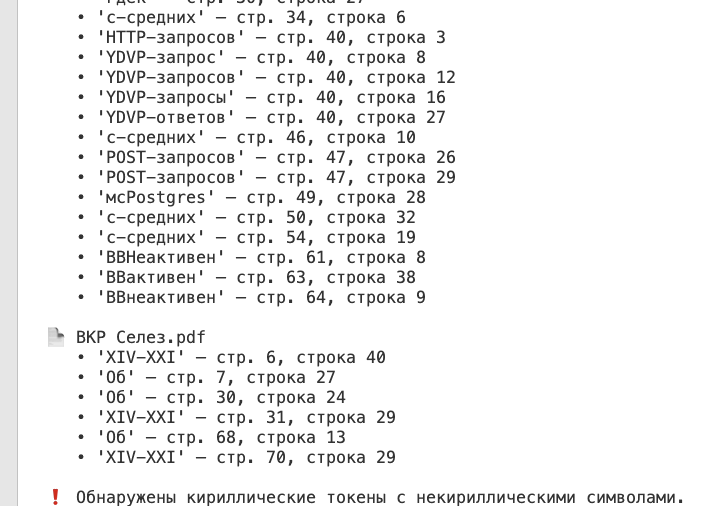
\includegraphics[width=1\textwidth]{images/aa-1.png}
	\caption{результаты решения сгенерировано с помощью Qwen Coder}
	\label{fig:ris1}
\end{figure}

\begin{figure}[H]
	\centering
	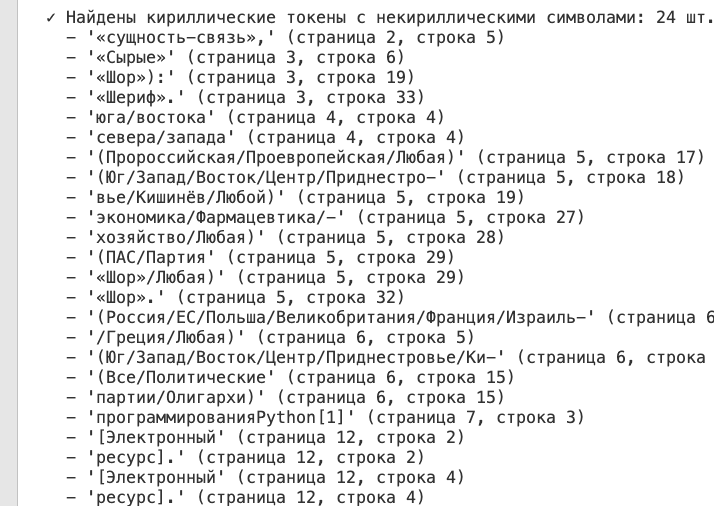
\includegraphics[width=1\textwidth]{images/aa-2.png}
	\caption{результаты решения сгенерировано с помощью DeepSeek}
	\label{fig:ris2}
\end{figure}

\begin{figure}[H]
	\centering
	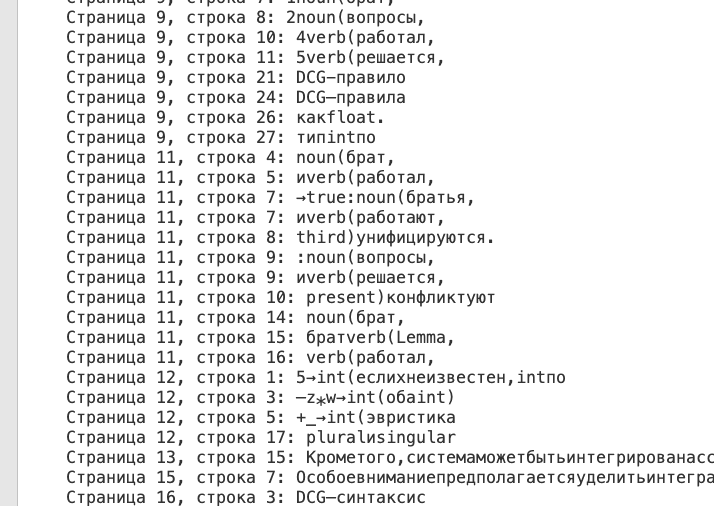
\includegraphics[width=1\textwidth]{images/aa-3.png}
	\caption{результаты решения сгенерировано с помощью ChatGPT 5.1}
	\label{fig:ris3}
\end{figure}

Тестирование алгортма, реализованного с помощью DeepSeek демонстрируется в таблице~\ref{tab:deepseek_errors} в приложении Б.
Тестирование алгортма, реализованного с помощью Qwen демонстрируется в таблице~\ref{tab:qwen_errors} в приложении Б.
Тестирование алгортма, реализованного с помощью ChatGPT 5.1 демонстрируется в таблице~\ref{tab:gpt_errors} в приложении Б.